%----------------------------------------------------------------------------------------
%	PACKAGES AND OTHER DOCUMENT CONFIGURATIONS
%----------------------------------------------------------------------------------------

\documentclass{article}

\usepackage{lastpage} % Required to determine the last page for the footer
\usepackage{extramarks} % Required for headers and footers
\usepackage{graphicx} % Required to insert images
\usepackage{gensymb}
\usepackage{hyperref}

\linespread{1.1} % Line spacing
\usepackage[total={6in, 9in}]{geometry}

\setlength\parindent{0pt} % Removes all indentation from paragraphs



\begin{document}
\title{Advanced Computer Graphics\\ Coursework 2}
\author{Terence Tse, Zhou Yu \\ Team JT}
\maketitle
\newpage

\section{Part 1: Fresnel reflectance}
Using the equations outlined in the notes for Fresnel reflectance,
the graph depicting parallel and perpendicular components of air to glass
(or some other material with a refraction index of 1.5)
which was a refraction index of 1.0 to 1.5 and can be seen in Figure 1. The
graph of Fresnel Reflectance from glass to air (1.5 to 1.0) is shown in 
Figure 2. The curve for Schlick's approximation of Fresnel
reflectance is seen in Figure 3. These can all be found in the "part1" folder
in the pictures folder of the attached files.\\
\\
From air to glass, we took the parallel component measurements and found
Brewster's angle to be \texttt{0.9837 radians} ($56.3636\degree$).

\begin{figure}[h]
	\centering
	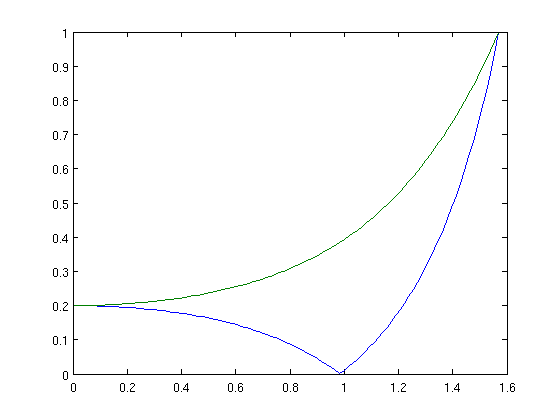
\includegraphics[scale=0.5]{pics/part1/air2glass.png}
	\caption{From a 1.0 index of refraction to 1.5}
\end{figure}

From glass to air, we took the parallel component measurements and from here
could owrk out the critical angle to be \texttt{0.7299 radians} 
($41.8182\degree$).

\begin{figure}[h]
	\centering
	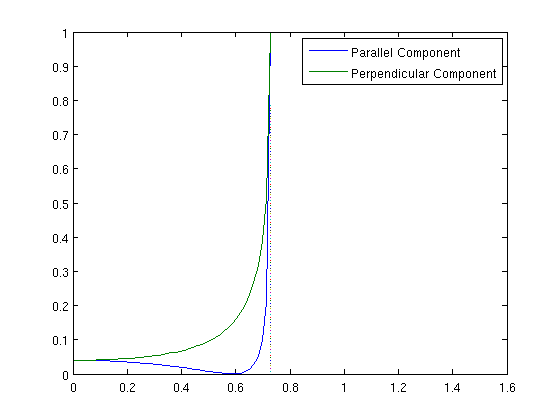
\includegraphics[scale=0.5]{pics/part1/glass2air.png}
	\caption{From a 1.5 index of refraction to 1.0}
\end{figure}

\newpage

Finally, with Schlick's approximation, we made sure to use the reflectance
of normal incidence from the air to glass Fresnel reflectance graph which 
was $2.0$.

\begin{figure}[h]
	\centering	
	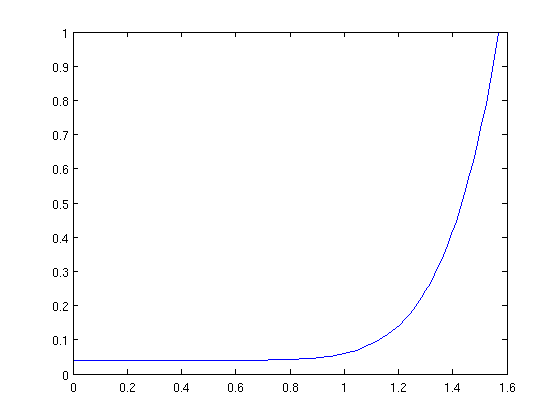
\includegraphics[scale=0.5]{pics/part1/Schlick.png}
	\caption{From a 1.0 index of refraction to 1.5}
\end{figure}


\section{Part 2: Environment Map(EM) sample generation}
The samples we took from the environment map can be see in 
\texttt{pics/part2/sample*.pfm} and \texttt{pics/part2/sample*.ppm} in the 
attached files. For each sample pixel, we have surrounded it with a $9$ pixel 
neighbourhood for better visualisation. 
\\
We have done sampling with the number of samples, N, being 64, 256 and 1024.
These are "Sampling64.ppm", "Sampling256.ppm" and "Sampling1024.ppm". We have
gamma corrected these too.

\section{Part 3: Environment Map(EM) Sphere Rendering}



\section{Part 4: Rendering a Sphere with Grace EM and PBRT}
Albedo was set at 1.0 and the three sphere can be seen in the
"part4" folder of the "pics" folder attached. These are the
.pfm and .ppm images named "simplesphere8", 
"simplesphere16" and "simplesphere32" for the 8,16, and
32 sample sampling methods.
As we can see from these images the general amount of noise 
decreased quite noticeably from 8 to 16 samples and again 
decreased from 16 to 32 but less noticeably.

\end{document}
